\documentclass{plantilla-manual-usuario-en}

\autor{PRYADES Soluciones Informáticas SL}
\proyecto{Teleradiología en la Nube}
\logotipo{images/imedig-logo.jpg}
\title{Manual de Usuario}
\company{images/pryades-logo.png}
\date{02/09/2015}

\begin{document}

\frontmatter

\maketitle

\newpage

\tableofcontents

\mainmatter

\section{3G gateway configuration for Teleradiology}

To setup the teleradiology service available for a radiology station the IMEDIG 3G gateway must be configured per the following instructions. Images transmission will take place as shown on figure \referencia{esquemaConexion}.

\figura{1}{images/esquema-conexion-en.png}{Gateway connection diagram}{esquemaConexion}{}

Connect radiology station with IMEDIG 3G Gateway using the crossover cable included in the package. 

IMEDIG 3G gateway is configured, by default, with one physical connection that uses two logical network address. One logical address will be used to do the connection with radiology station and the other should be used only for configuration management.

The default logical address for IMEDIG 3G gateway configuration is:

\begin{itemize}
\item IP address: 192.168.254.253 
\item Gateway: 255.255.255.0
\end{itemize}

It is possible that the radiology station, by its network configuration, do not have access to addresses on the 192.168.254.X segment. In this case, you should add to the station a new logical IP address located inside this segment. For Windows XP you can do this applying the following steps: 

\begin{itemize}
\item Open ``Networks connections'' folder.
\item Click the right mouse button upon Local network item and select the option ``Properties''
\item Select tab ``Advanced options'' in the window that shows up.
\item Below the list entitled ``IP Address'' press the button ``Add'' and type one address in the range 192.168.254.X.
\end{itemize}

Verify the connection works using the system command ``ping 192.168.254.253''. 

\subsection{Access to the gateway configuration interface} \label{labelInterfaceConfiguracion}

Once the logical address for IMEDIG 3G gateway is operational you can proceed to set up the correct parameters for the local intranet. Open a web browser and type the URL:

http://192.168.254.253/imedig/config

An authentication screen will show up where you must introduce:

\begin{itemize}
\item User: root
\item Password: root
\end{itemize}

Figure \referencia{figuraConfiguracion} shows the data that must be set up for local, administration and 3G connections.

\figura{1}{images/configuracion-en.png}{Gateway configuration}{figuraConfiguracion}{} 

You must introduce a local IP address for the IMEDIG 3G gateway in the Local Connection column.  It must be in the same segment address where the radiology station is placed. Address and Mask are the mandatory parameters. The others parameters of this column are optional and they should not be filled for the case when the teleradiology connection will be done through 3G.

\subsection{3G connection configuration}

You must set up the appropiated parameters for 3G connection depending on the mobile phone company that provides connection. The following table shows known values tested for connection through some mobile phone companies. The correct values for other companies not listed must be found contacting their client support branch.


\begin{center}
  \begin{tabular}{ | l | l | l | l | l |}
    \hline
    Company & APN & Phone number & User & Password \\ \hline
	T-Mobile USA & epc.tmobile.com & \#99* & user & pass \\ \hline
	Movistar Spain & movistar.es & \#99* & movistar & movistar \\ \hline
	Movistar Guatemala & internet.movistar.gt & \#99* & movistargt & movistargt \\ \hline
	Orange Spain & orangeworld & \#99* & orange & orange \\ \hline
  \end{tabular}
\end{center}

Set tabulated parameters and press the Apply button. Then press the Reboot button so that the gateway could restart the operations using the new configuration data. The restart may take a few minutes until the gateway is operable again.

\subsection{Configuration of IMEDIG gateway as DICOM entity}

The radiology station must have knowledge of IMEDIG 3G gateway as a DICOM entity in order to be able to transmit images to it. Introduce in the DICOM configuration of the radiology station the data of IMEDIG 3G gateway as storage entity as per following guidelines:

\begin{itemize}
\item address: the one you have assigned in the steps of section \referencia{labelInterfaceConfiguracion}. Example: 192.168.1.253
\item AETitle: DCM4CHEE
\item port: 11112
\end{itemize}

Prove connectivity between radiology station and IMEDIG 3G gateway. You may use tools such as PING or DICOM ECHO that are installed on it.

\subsection{Setting of the 3G modem}

Make sure that the SIM card you will install on the 3G modem do not have PIN request enabled. You can disable this feature by installing the SIM first on a cell phone and accessing the configuration menu.

Install the SIM card on the 3G modem you received woth the package and plug the modem  on a free USB port of the station. The led of the 3G modem will flash as it establishes connection. It flashes first in red light and then, in green light. The led stops flashing when the connection has been set  and keeps a still green light. If it keeps flashing with red light during a long time make sure that it has not the PIN request enabled. If the situation persists, contact the support personnel. 

\subsection{Remote connection}

Once the IMEDIG 3G gateway has established a succesfull internet connection, it will record the dynamic IP address received from the supplier. It will be accessible through the URL:

http://viewerXXX.lomisa.es/imedig/viewer

where XXX letters must be replaced with the numbers printed on the label you can found on the front of the computer box.

The address domain ``viewerXXX.lomisa.es'' should be accessible in few minutes. Since the availability of the domain depends on propagation through DNS servers, eventually it may take more time until the access is enabled.  

The access to the URL previously given can be tested on an internet browser like Chrome, Firefox, Safari or Internet Explorer 9+.

\subsection{Requirements for accessing internet for 3G IMEDIG gateway}

For 3G IMEDIG gateway having a proper internet connection to provide its services efficiently it is required an enabled SIM card for a local mobile operator with an internet plan with a steady speed regardless of traffic volume. Data plans in some countries provide high speed for 1 GB per month and then speed is reduced to a figure not good for image transmission. Special care should be taken into account selecting the data plan to avoid that situation.  

\subsection{Requirements for remote access equipment}

To remote access to images stored in 3G IMEDIG Gateway a computer with the following minimal characteristics is required:

\begin{itemize}
\item 2 GHz CPU Speed
\item 1280 x 1024 pixels resolution monitor, suitable for medical diagnosis
\item 2 GB RAM
\item Firefox, Chrome, Safari, Internet Explorer 9 or Opera internet Browser
\item 1 Mbps internet connection speed
\item Windows XP or higher, Linux or Macintosh operating system
\end{itemize}

\section{Starting the application}

IMEDIG gateway for teleradiology is started by introducing the following link on a web browser (it is compatible with Chrome, Safari, Firefox, Internet Explorer 9+):

http://viewerXXX.lomisa.es/imedig/viewer

Accesing \href{http://www.lomisa.es/imedig/viewer}{http://www.lomisa.es/imedig/viewer} a demo of the application could be visualized. A few images are available in this demo for testing.

\section{User authentication}

An identification form will be shown on the initial window (see figure \referencia{figuraLogin}) where user should type login and password. 

\figura{0.5}{images/login-en.png}{User authentication form}{figuraLogin}{}

If your application has been started from a trusted application in which the user has already been authenticated or has been configured not to use authentication, the previous step is not necessary. Instead of a window with the identification form, a window for selecting studies will be shown. This window is described in section \referencia{seccionAbrir}

\section{Main window}

Three areas form the application main window:

\begin{itemize}
\item Study cards.
\item Images area. 
\item Controls bar.
\end{itemize}

\figura{1}{images/estructura-interfaz.png}{User interface structure}{figuraEstructuraInterfaz}{}

\subsection{Study cards}

The figure \referencia{figuraEstructuraInterfaz} shows that \italics{Study cards} area appears in the left side of main window. Color boxes with icons and information about selected studies are shown inside this area.

Icons corresponding to the images included in each series from the study are shown inside each card. If there is no enough space in the \italics{Study cards} area to show all icons of images then a scroll bar will appear in its right side.

The heading of a study card shows initials of patient name, date of the study and patient's  identifier. The patient's full name is shown when mouse cursor is drag over initials and the image modality is shown when mouse cursor is drag over icons of images.

If left button of mouse is clicked on an icon of an image, then this image is visualized on the \italics{Images area} with better resolution.

\subsection{Images area}

At the central part of user interface is located the \italics{Images area} as can be seen at figure \referencia{figuraEstructuraInterfaz}. The image which icon is currently selected will be visualized in this area with enhanced detail. 

\subsection{Controls bar}
The \italics{Controls bar} area appears in the upper part of left side of main window. This bar includes control buttons corresponding to operations that can be executed on images. A hint text describing the related operation will be shown when the mouse cursor is drag over each button:

\begin{itemize}
\item Open: Open studies that are selected in the resulting list that is displayed after a filtered search.
\item Close: Close studies currently opened.
\item None operation: Cancel the operation currently selected leaving no operation active.
\item Zoom: Activate zoom operation to be applied over interest region from the image.
\item Brightness and contrast: Modify brightness and contrast levels of the image in order to enhance its visual quality.
\item Undo: Undo the effect of the operation more recently applied.
\item Measure length: To measure length between to image points. 
\item Measure angle: To measure angle between two lines superposed over the image. 
\item Exit: End the user session currently opened.
\end{itemize}

\section{Operations description}
Operations that modify visual characterictics of the image are executed on the server and its result is downloaded to your browser. The quickness for seeing the modified image on your screen will depend on several factors such server workload, net overload, etc. In cases where it is required to repeat the execution of an operation several times, a correct strategy must be applied in order to avoid unnecessary server workload and to reduce the overall time consumed. In order to optimized internet traffic, results of some operations are not available until left mouse button is released.

A detailed description of each operation is provided next.

\subsection{Open}
\label{seccionAbrir}

The user can select the studies he wants to be opened using this operation. It is activated when left mouse button is pressed upon icon 
\includegraphics[scale=0.5]{images/open.png}. The search form shown on figure \referencia{figuraAbrirEstudios} will come out to the screen after clicking the mouse.  

\figura{1}{images/abrir-estudios1-en.png}{Form to search and retrieve studies from the PACS server}{figuraAbrirEstudios}{}

The following list give a brief description of search criteria that can be introduced into the form:

\begin{itemize}
\item Name: search studies with the patient's name containing the introduced text. 
\item Identifier: search studies with the patient's identifier containing the introduced text. 
\item Type: The result of the search will include those studies whose modality match the one selected on the list. 
\item Date: search studies made in a date with a difference with respect to the current date that does not exceed the amount selected in the list. 
\end{itemize}

If the input line of some criteria is empty it is assumed that all studies match the corresponding search criteria. To execute the search the left mouse button must be pressed upon the button 
\includegraphics[scale=0.5]{images/buscar.png}.

The first, previous, next or last page of the table can be accessed 
using the icons with arrows shown above the table of results. 
The current page number appears between previous and next page arrows, followed by the total number of pages

The selection of a study from the table is done by clicking the left mouse upon the check box in the first column of the study row. After that, the left mouse button must be pressed on the button \italics{Open}.
\subsection{Show reports}

When the study card is shown including an icon such as 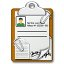
\includegraphics[scale=0.3]{images/report-icon.jpeg} it means that the study contains a report made previously by a radiologist using a diagnostic application. A window showing the report content will be opened if left mouse button is clicked upon the report icon(see figure \referencia{figuraInformes}). Inside the report could be found text lines describing observations written by the radiologist along with some images for a possible diagnosis.

\figura{1}{images/mostrar-informe-en.png}{Window showing report content}{figuraInformes}{}

\subsection{Close}

Close all study cards and images opened. It is inactivated when no study is open. It is executed when left mouse button is pressed upon 
\includegraphics[scale=0.5]{images/close.png}

\subsection{Zoom}

This operation is activated by pressing the left mouse button upon the icon 
\includegraphics[scale=0.5]{images/magnifier.png} in the \italics{Controls bar}. It can be used to see an image region with higher detail.

The region of interest for the zoom will be framed inside a rectangle that will be drawn above the image while the user drag the mouse over it. Move the mouse to a vertex of the rectangle and press its left button. Then, without releasing the button, drag it until reaching the opposite vertex. Release the left button at the opposite vertex.

The zoomed region, with correct aspect ratio, will be shown on the \italics{Images area} of the application.If more detail is desire, then the operation could be applied again. Figure \referencia{figuraZoom} shows the 
zoomed rectangle from a region of the image on figure \referencia{figuraEstructuraInterfaz}.

\figura{1}{images/figura-zoom.png}{Zoomed image region}{figuraZoom}{}

\subsection{Brightness and Contrast}

Modify brightness and contrast in the selected image. It is activated by pressing the left mouse button upon the icon 
\includegraphics[scale=0.5]{images/contrast.png}.

To execute the operation, place the mouse on any point of the image that you wish to modify. Press the left button and, without releasing it, move the mouse toward any direction. The properties of the image will change according to the following criteria:

\begin{itemize}
\item A movement to the right will decrease contrast. 
\item A movement to the left will increase contrast. 
\item A movement down will decrease brightness.
\item A movement up will increase brightness.
\end{itemize}

The resulting image (with the brigtness and contrast changed) will be shown when the left mouse button is released.

\subsection{Undo}

Undoes the effect of the operation more recently applied. The modified image will be displayed as it was before applying the operation. This operation is activated by pressing the left mouse button upon the icon 
\includegraphics[scale=0.5]{images/undo.png}. The icon will be shown as inactive if there is no operation to be undone.

\subsection{Measure length}

Use this operation to measure the length between two image points. It is activated by pressing the left mouse button upon the icon 
\includegraphics[scale=0.5]{images/distance.png}. 

Press the left mouse button upon one of the two points whose inner distance you wish to measure. Move the mouse toward the other point without releasing the button. A line will be superposed above the image showing the line whose length is being measured. Release the left button when reaching the other point. An annotation with the measure taken will be attached to the line as shown on the figure \referencia{figuraMediciones}.

\figura{1}{images/figura-mediciones-en.png}{Measuring length and angle}{figuraMediciones}{}

Taking a measure requires that calibration data related to length be present inside image data. If this type of data is absent then the button for measuring length will not be active. 

\subsection{Measure angle}

With this operation the angle between two lines superposed over the image can be measured. It is activated by pressing the left mouse button upon the icon 
\includegraphics[scale=0.5]{images/angle.png}

To obtain this measurement the user must draw two lines above the image. The minor angle formed between this two lines will be the resulting measure. To plot each line place the mouse in one extreme, press its left button, and move toward the other extreme holding the button pressed. Release the button in the other extreme. When plotting of the second line is finished an annotation with the minor angle between the two lines is shown attached to this second line as shown in the fgiure \referencia{figuraMediciones}.

\subsection{No operation}

Cancel the operation currently selected leaving no operation activated. It is executed by pressing the left mouse button upon the icon 
\includegraphics[scale=0.5]{images/cursor.png}. Mouse click upon the selected image has no 
effect when this operation is active.

\subsection{Exit}

End the user session currently opened. All images currently open will be closed and the authentication form came up to the screen (see figure \referencia{figuraLogin}). This happens when the left mouse button is clicked upon the icon 
\includegraphics[scale=0.5]{images/exit.png}. If the application had been run without using authentication then you must close the browser to exit from it.

\clearpage

\section{Contact}

To get more information please contact with:

PRYADES Soluciones Informáticas SL\\*
c/ La Fragua 5\\*
28260, Galapagar, Madrid\\*
Spain\\*
Ph: +34 918 586 353\\*
Correo: direccion@pryades.com\\*

\end{document}
